\documentclass[journal,12pt,twocolumn]{IEEEtran}
\usepackage{amsthm}
\allowbreak
\usepackage{setspace}
\usepackage{gensymb}
\singlespacing
\usepackage[cmex10]{amsmath}
\usepackage{caption}
\usepackage{amsthm}

\DeclareUnicodeCharacter{2212}{-}
\usepackage{tikz}
\usepackage{pgfplots}

\usepackage{mathrsfs}
\usepackage{txfonts}
\usepackage{stfloats}
\usepackage{bm}
\usepackage{cite}
\usepackage{cases}
\usepackage{subfig}

\usepackage{longtable}
\usepackage{multirow}

\usepackage{enumitem}
\usepackage{mathtools}
\usepackage{steinmetz}
\usepackage{tikz}
\usepackage{circuitikz}
\usepackage{verbatim}
\usepackage{tfrupee}
\usepackage[breaklinks=true]{hyperref}
\usepackage{graphicx}
\usepackage{tkz-euclide}
\graphicspath{ {./images/} }
\usetikzlibrary{calc,math}
\usepackage{listings}
    \usepackage{color}                                            %%
    \usepackage{array}                                            %%
    \usepackage{longtable}                                        %%
    \usepackage{calc}                                             %%
    \usepackage{multirow}                                         %%
    \usepackage{hhline}                                           %%
    \usepackage{ifthen}                                           %%
    \usepackage{lscape}     
\usepackage{multicol}
\usepackage{chngcntr}

\DeclareMathOperator*{\Res}{Res}

\renewcommand\thesection{\arabic{section}}
\renewcommand\thesubsection{\thesection.\arabic{subsection}}
\renewcommand\thesubsubsection{\thesubsection.\arabic{subsubsection}}

\renewcommand\thesectiondis{\arabic{section}}
\renewcommand\thesubsectiondis{\thesectiondis.\arabic{subsection}}
\renewcommand\thesubsubsectiondis{\thesubsectiondis.\arabic{subsubsection}}


\hyphenation{op-tical net-works semi-conduc-tor}
\def\inputGnumericTable{}                                 %%

\lstset{
%language=C,
frame=single, 
breaklines=true,
columns=fullflexible
}
\begin{document}


\newtheorem{theorem}{Theorem}[section]
\newtheorem{problem}{Problem}
\newtheorem{proposition}{Proposition}[section]
\newtheorem{lemma}{Lemma}[section]
\newtheorem{corollary}[theorem]{Corollary}
\newtheorem{example}{Example}[section]
\newtheorem{definition}[problem]{Definition}

\newcommand{\BEQA}{\begin{eqnarray}}
\newcommand{\EEQA}{\end{eqnarray}}
\newcommand{\define}{\stackrel{\triangle}{=}}
\bibliographystyle{IEEEtran}
\raggedbottom
\setlength{\parindent}{0pt}
\providecommand{\mbf}{\mathbf}
\providecommand{\pr}[1]{\ensuremath{\Pr\left(#1\right)}}
\providecommand{\qfunc}[1]{\ensuremath{Q\left(#1\right)}}
\providecommand{\sbrak}[1]{\ensuremath{{}\left[#1\right]}}
\providecommand{\lsbrak}[1]{\ensuremath{{}\left[#1\right.}}
\providecommand{\rsbrak}[1]{\ensuremath{{}\left.#1\right]}}
\providecommand{\brak}[1]{\ensuremath{\left(#1\right)}}
\providecommand{\lbrak}[1]{\ensuremath{\left(#1\right.}}
\providecommand{\rbrak}[1]{\ensuremath{\left.#1\right)}}
\providecommand{\cbrak}[1]{\ensuremath{\left\{#1\right\}}}
\providecommand{\lcbrak}[1]{\ensuremath{\left\{#1\right.}}
\providecommand{\rcbrak}[1]{\ensuremath{\left.#1\right\}}}
\theoremstyle{remark}
\newtheorem{rem}{Remark}
\newcommand{\sgn}{\mathop{\mathrm{sgn}}}
\providecommand{\abs}[1]{$\left\vert#1\right\vert$}
\providecommand{\res}[1]{\Res\displaylimits_{#1}} 
\providecommand{\norm}[1]{$\left\lVert#1\right\rVert$}
%\providecommand{\norm}[1]{\lVert#1\rVert}
\providecommand{\mtx}[1]{\mathbf{#1}}
\providecommand{\mean}[1]{E$\left[ #1 \right]$}
\providecommand{\fourier}{\overset{\mathcal{F}}{ \rightleftharpoons}}
%\providecommand{\hilbert}{\overset{\mathcal{H}}{ \rightleftharpoons}}
\providecommand{\system}{\overset{\mathcal{H}}{ \longleftrightarrow}}
	%\newcommand{\solution}[2]{\textbf{Solution:}{#1}}
\newcommand{\solution}{\noindent \textbf{Solution: }}
\newcommand{\cosec}{\,\text{cosec}\,}
\providecommand{\dec}[2]{\ensuremath{\overset{#1}{\underset{#2}{\gtrless}}}}
\newcommand{\myvec}[1]{\ensuremath{\begin{pmatrix}#1\end{pmatrix}}}
\newcommand{\mydet}[1]{\ensuremath{\begin{vmatrix}#1\end{vmatrix}}}
\numberwithin{equation}{subsection}
\makeatletter
\@addtoreset{figure}{problem}
\makeatother
\let\StandardTheFigure\thefigure
\let\vec\mathbf
\renewcommand{\thefigure}{\theproblem}
\def\putbox#1#2#3{\makebox[0in][l]{\makebox[#1][l]{}\raisebox{\baselineskip}[0in][0in]{\raisebox{#2}[0in][0in]{#3}}}}
     \def\rightbox#1{\makebox[0in][r]{#1}}
     \def\centbox#1{\makebox[0in]{#1}}
     \def\topbox#1{\raisebox{-\baselineskip}[0in][0in]{#1}}
     \def\midbox#1{\raisebox{-0.5\baselineskip}[0in][0in]{#1}}
\vspace{3cm}
\title{AI1103: Assignment 3}
\author{Tanmay Garg \\CS20BTECH11063 EE20BTECH11048}
\maketitle
\newpage
\bigskip
\renewcommand{\thefigure}{\theenumi}
\renewcommand{\thetable}{\theenumi}



Download all python codes from 
\begin{lstlisting}
https://github.com/tanmaygar/AI-Course/blob/main/Assignment3/codes/GATE-2007-(MA)-Q14.py
\end{lstlisting}
%
and latex-tikz codes from 
%
\begin{lstlisting}
https://github.com/tanmaygar/AI-Course/blob/main/Assignment3/Assignment3.tex
\end{lstlisting}
\section*{Problem GATE 2007 (MA), Q. 14: }
Let $X$ and $Y$ be jointly distributed random
variables having the joint probability
density function
\[
f(x,y) = \begin{cases}
            \frac{1}{\pi}, &\text{if}\quad x^2 + y^2 \leq 1\\
             0, &\text{otherwise}\\
            \end{cases}
\]
Then $\pr{Y > \text{max}(X,-X)}$ is

\section*{Solution:}
The pdf of $X$ and $Y$ are:
\begin{align}
    f_X(x)&=\int_{-\infty}^{\infty}f(x,y)dy\\
    &=\int_{-\sqrt{1-x^2}}^{\sqrt{1-x^2}}\frac{1}{\pi}dy\\
    &=\frac{2\sqrt{1-x^2}}{\pi}
\end{align}
\begin{align}
    f_Y(y)&=\int_{-\infty}^{\infty}f(x,y)dx\\
    &=\int_{-\sqrt{1-y^2}}^{\sqrt{1-y^2}}\frac{1}{\pi}dx\\
    &=\frac{2\sqrt{1-y^2}}{\pi}
\end{align}
The cdf of $Y$ is:
\begin{align}
    F_Y(y)&=\int_{-\infty}^{y}f_Y(y)dy\\
    &=\int_{-1}^{y}\frac{2\sqrt{1-y^2}}{\pi}dy\\
    &=\frac{2}{\pi}\left(\dfrac{\sin^{-1}{y} + y\sqrt{1-y^2}}{2} + \frac{\pi}{4}\right)
\end{align}
The value of $\pr{-X<Y<X}$ is:
\begin{align}
\pr{-X<Y<X} &=F_Y(X)-F_Y(-X)\\
 &=\frac{2}{\pi}\left(\sin^{-1}{X} + X\sqrt{1-X^2}\right)
\end{align}

Integrating our probability over all of $X$ we get the value of $\pr{Y>\text{max}(X,-X)}$:
\begin{align}
 &=\int_{-\infty}^{\infty}f_X(x)\pr{-x<Y<x}dx\\
    &=\left(\frac{2}{\pi}\right)^2\int_0^1\sqrt{1-x^2}\left(\sin^{-1}{x} + x\sqrt{1-x^2}\right)dx
\end{align}
Substituting
\begin{align} 
u &= \sin^{-1}{x} + x\sqrt{1-x^2}\\
\frac{du}{dx} &= 2\sqrt{1-x^2}\\
&=\left(\frac{2}{\pi}\right)^2\int_0^{\frac{\pi}{2}}\frac{u}{2}du\\
&=\left(\frac{2}{\pi}\right)^2\left(\frac{u^2}{4} \bigg |_0^{\frac{\pi}{2}}\right)\\
&=\left(\frac{2}{\pi}\right)^2\left(\frac{\pi^2}{16} - 0\right)\\
    &=\frac{4\cdot{\pi}^2}{{\pi}^2\cdot16}\\
    &=\frac{1}{4}
\end{align}
The probability for:
\begin{align}
    \pr{Y>\text{max}(X,-X)} = \frac{1}{4}
\end{align}
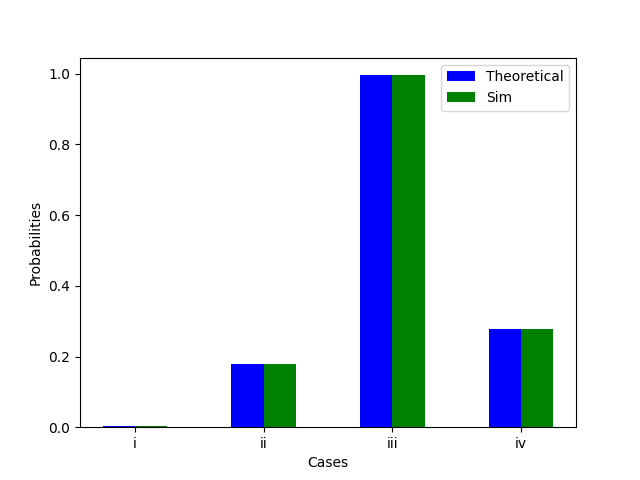
\includegraphics[width=0.45\textwidth]{Figure_1.png}
\end{document}